\chapter{Primordial Black Holes}
\hspace{0.5cm}In the year 1971 Hawking \cite{1971MNRAS.152...75H} made a groundbreaking discovery that highly overdense regions of inhomogeneities in the primordial universe can undergo gravitational collapse to form BH's. This initiated the modern mechanism of formation and there have been several mechanisms proposed for the formation of PBH like primordial inhomogeneities\cite{1975ApJ...201....1C}, collapse from scalar -invariant fluctuation \cite{1975ApJ...201....1C}, collapse in the matter-dominated era, collapse in inflationary fluctuations, collapse at the QCD phase transition, the collapse of cosmic loops, collapse through bubble collision.

\hspace{0.5cm} Previously, we discussed how inflation causes the Hubble horizon to shrink on a comoving scale, enabling quantum fluctuations to transform into classical density perturbations as they exit the horizon. As inflation comes to an end, the horizon expands, and these perturbations begin to re-enter the horizon. As these large perturbations re-enter, they create regions of high density that can collapse to form PBHs in the early radiation-dominated universe. To determine whether a particular region of the early universe has the potential to collapse and form PBHs, researchers typically compare either the region's density or curvature to a specific threshold value. This threshold value is often derived from numerical simulations and serves as a criterion for predicting PBH formation. In the following section, we will follow the approach discussed in Ref. \cite{Sasaki_2018}, which combines the traditional method based on density contrast with the newer approach based on curvature perturbations, to provide a comprehensive overview of PBH formation in a simple way.

%%%%%%%%%%%%%%%%%%%%%%%%%%%%%%%%%%%%%%%%%%%%%%%%%%%%%%%%%%%%%%%%%%%%%%%%%%%
\section{Simple Physical Model for PBH formation}

In the early Universe after inflation, as discussed in Chapter 1 the background spacetime can be described by the spatially-flat Friedmann-Lemaitre-Robertson-Walker (FLRW) metric, which assumes a homogeneous and isotropic space (\ref{eq:1.2} - \ref{eq:1.4}). We can obtain the background Friedmann equation from the Einstein equation 
\begin{align}
    \left(\frac{\dot{a}}{a}^2\right) = \frac{8\pi G}{3} \bar{\rho}(t), \label{3.1}
\end{align}
 

\hspace{0.5cm}We consider a locally perturbed region against this background that would eventually collapse into a black hole. Such a region is a rare occurrence in space and can be approximated by a spherically symmetric region of positive curvature. As matter within the region becomes highly concentrated, the curvature of spacetime becomes large. The collapse is highly symmetric, so we assume that the curvature is concentrated around the centre of the region, and the geometry can be approximated by a spherically symmetric region of positive curvature.
 The comoving size of the region is initially much larger than the Hubble horizon size, so we can apply the leading order spatial gradient expansion\footnote{ Gradient expansion is useful to study the evolution of cosmological perturbations on sufficiently large smoothing scales. The universe becomes locally (smaller than the smoothing scale and larger than the Hubble scale) homogeneous and isotropic (FRW).In brief, the gradient expansion is a systematic expansion in spatial derivatives of the perturbations. In the superhorizon limit, the perturbations are nearly constant, and the leading-order behaviour is determined by the zeroth-order term. However, on subhorizon scales, the perturbations are rapidly varying, and higher-order terms in the gradient expansion become important. By truncating the gradient expansion at a certain order, we can approximate the behaviour of the perturbations on a certain range of scales.} \cite{Lyth_2005},\cite{Shibata_1999},\cite{Harada_2015}.\\
 
 The metric can be expressed as
 \begin{align}
     ds^2=-dt^2+a(t)^2e^{2\zeta(r)}\delta_{ij}dx^idx^j ,\ \label{3.2}
 \end{align} 
 where $\zeta>0$ and decreases to zero as $r \rightarrow \infty$. This metric is consistent with the metric on comoving slices(the one orthogonal to the comoving worldlines) on superhorizon scales(the uniform-density, uniform-expansion, and comoving slices coincide in the large scale limit)\footnote{For detail description refer to \cite{Lyth_2005},\cite{Harada_2015}}, where $\zeta$ is the conserved comoving curvature perturbation.\\
 The metric can be transformed into a locally closed universe with the metric \begin{align*}
     ds^2=-dt^2+a(t)^2\left[\frac{dR^2}{1-K(R)R^2}+R^2\left(d\theta^2+\sin^2\theta d\varphi^2\right)\right]
 \end{align*}, 
 where the coordinates $r$ and $R$ are related to each other as $R=re^{\zeta(r)}$, and $K$ is given by
 \begin{align}
     K=-\frac{\zeta^{\prime}(r)}{r}\frac{2+r\zeta^{\prime}(r)}{e^{2\zeta(r)}},\ \label{3.3}
 \end{align}
this equation shows the relation between $K$ in terms of spatial curvature perturbation $\zeta(r)$
One can use the gradient expansion on superhorizon scales\cite{Shibata_1999, Polnarev:2006aa}. Only the first non-vanishing terms in the power expansion of the small parameter $\epsilon \ll 1$, where $\epsilon$ is defined as the ratio between the Hubble radius and the length scale of the perturbation, are taken into consideration by this approximation. The energy density profile can be expressed as follows in this limit\cite{Harada_2015, Musco:2018rwt}:
\begin{align}
    \delta = \frac{\delta \rho}{\bar{\rho}} \equiv \frac{\rho(r, t)-\bar{\rho}(t)}{\bar{\rho}(t)}=-\frac{1}{a^2 H^2} \frac{4(1+w)}{5+3 w} e^{-5 \zeta(\hat{r}) / 2} \nabla^2 e^{\zeta(\hat{r}) / 2} \label{3.4}
\end{align}

where $H(t)=\dot{a}(t) / a(t)$ is the Hubble parameter, $\bar{\rho}$ is the mean background energy density and $\nabla$ denote differentiation with respect to $\hat{r}$. The parameter $w$ is the coefficient of the equation of state $p=w \rho$ relating the total (isotropic) pressure $p$ to the total energy density $\rho$, which takes the value $w=1 / 3$ in a radiation-dominated universe.

Let us provide a simplified analytical argument showing the characteristic value of the threshold for PBH collapse \cite{Sasaki_2018}. The intrinsic 3-curvature of the $t=\text{const.}$ hypersurface is given by 
\begin{align*}
    R^{(3)}=\frac{K}{a^2}\left(1+\frac{d\ln K(R)}{3d\ln R}\right) ,\ 
\end{align*}
Ignoring the spatial derivative of $K$ in the leading order gradient expansion, the Hamiltonian constraint (time-time component) is given by
\begin{align}
    H^2+\frac{K(r)}{a^2}=\frac{8\pi G}{3}\rho,\label{3.5}
\end{align}
 which is equivalent to the Friedmann equation describing the evolution of a spatially curved universe. This can be regarded as the Hamiltonian constraint on the comoving hypersurface or on the uniform Hubble hypersurface, on which the expansion rate is spatially homogeneous and isotropic which is the condition for FRW. 

From the above equation, we can define the density contrast on the comoving hypersurface by
\begin{align}
    \delta:=\frac{\rho-\bar{\rho}}{\bar{\rho}}=\frac{3 K}{8 \pi G \bar{\rho} a^2}=\frac{K}{H^2 a^2}\label{3.6}
\end{align}


As we saw previously that during the radiation-dominated era $\bar{\rho}(t) \propto a^{-4}$ (Eq. \ref{eq:1.24})  therefore $\delta$ is vanishingly small initially, so it is the curvature perturbation that influences the density perturbation which is consistent with our previous discussion.

As the universe evolves, the value of $\delta$ increases and approaches unity. If we disregard the spatial variation of $K$, a universe with positive curvature ($K>0$) will eventually cease expanding and collapse in on itself. This occurs when $3 K / a^2 = 8 \pi G \rho$, which is when the comoving scale of the positively curved region becomes comparable to the Hubble horizon scale. At this point, the separate universe approximation breaks down, and the equivalence between the comoving and uniform Hubble slices is no longer valid. However, it is still reasonable to expect that equation \ref{3.5} can be used to obtain a qualitatively acceptable criterion for black hole formation. In fact, this approach has been validated by fully nonlinear numerical simulations.

We consider that the formation of black holes occurs at the epoch when the universe stops expanding i.e. $\delta = 1$. We can set this time as $t=t_c$. Since for perturbation smaller than the Jeans length the collapse is not feasible, we set the condition for collapse to be when $c_s^2 k^2 / a^2=H^2$ or $k^2 / a^2=3 H^2$ for $c_s^2=1 / 3$.

Namely, we have
\begin{align}
    1=\delta\left(t_c\right)=\frac{K}{k^2} \frac{k^2}{H^2 a^2}=\frac{K}{c_s^2 k^2} ,\ \label{3.7}
\end{align}
We can then identify $K$ with $c_s^2 k^2$ and obtain the criterion for black hole formation as follows: the comoving slice density contrast at the time when the scale of interest re-enters the Hubble horizon should be greater than $\delta_c=c_s^2$, i.e.,
\begin{align}
    \delta\left(t_k\right)=\frac{K}{H^2\left(t_k\right) a^2\left(t_k\right)}=\frac{c_s^2 k^2}{H^2\left(t_k\right) a^2\left(t_k\right)} \geq \delta_c=c_s^2=\frac{1}{3},\ \label{3.8}
\end{align}
where $t_k$ is the time at which k/a = H.
At this degree of approximation, the Jeans length($ R_{j} = c_{s} H^{-1}$) and the Hubble horizon cannot be distinguished. In general, it can be roughly estimated that the mass of the resulting PBH  is equal to the horizon mass at the time of formation i.e $M \sim M_{H} $.\\
We can use this to find an estimate of the time of formation $t_f$
\begin{align}
    M \sim M_{H} = \frac{4\pi}{3} \rho_{H} R_{H}^3 
    &= \frac{4\pi}{3} \frac{3H^2}{8 \pi G} \left(\frac{1}{H} \right)^3 = \frac{t_f}{G} \label{3.9}
\end{align}
where we used $H \propto \frac{1}{2t}$ during the radiation domination era. So we can get the simplest model which gives us an idea about the possible mass range of PBHs which is given by,
\begin{align}
    M \sim 
    \frac{t_f}{G} \sim 10^{15} \left(\frac{t}{10^{-23} s} \right)g \label{3.10}
\end{align}

The above discussion is a useful framework to understand the simplified physical model for the formation of PBH from primordial perturbations. Although this type of study effectively captures the essence of PBH formation, it is crucial to understand the significance of the various effects that were not taken into account in the discussion above. We will discuss this in the section \ref{limtiation}
%%%%%%%%%%%%%%%%%%%%%%%%%%%%%%%%%%%%%%%%%%%%%%%%%%%%%%%%%%%%%%%%%%%%%%%%%%%%

%%%%%%%%%%%%%%%%%%%%%%%%%%%%%%%%%%%%%%%%%%%%%%%%%%%%%%%%%%%%%%%%%
\section{PBH Abundance}
In this section, we will determine how to estimate the PBH's abundance. We will first introduce a parameter $\beta(M)$ (M is some mass-scale that is epoch dependent.) that represents the mass fraction of PBHs at the epoch of formation. The current density parameter $\Omega_{PBH}$ which is associated with unevaporated PBHs that form at a redshift $z$ is approximately related to $\beta$ by \cite{1975ApJ...201....1C}.
\begin{align}
    \Omega_{PBH} \simeq \beta\Omega_{r}(1+z)
    &\sim 10^6\beta\left( \frac{t}{1s}\right)^{-1/2} 
    \sim 10^{18}\beta \left(\frac{M}{10^{15}g }\right)^{-1/2},\ \label{3.11}
\end{align}

where we have used Eq.\ref{3.10} for the final form in terms of $ M > 10^{15}g$ (is considered as all the PBHs with mass below that would have been evaporated by now), $\Omega_{r} \sim 10^{-4}$  is the density parameter of the CMB. We get the $(1+z)$ factor because the radiation density scales as $(1+z)^4$, whereas the PBH density scales as $(1+z)^3$.Here we have also neglected the entropy production after the PBH formation. Let us look into a more precise formula \cite{PhysRevD.81.104019}:\\
\hspace{0.5cm}Previously it was shown the PBHs mass formed in the radiation-dominated epoch can be approximated as the horizon mass Eq. \ref{3.9}, at the formation, hence we have

\begin{align}
    M = \gamma M_{H|_{form}} = \gamma\frac{4\pi}{3}\rho_{form} H_{form}^{-3} =  \gamma\frac{4\pi}{3}\frac{3H^2_{form}}{8\pi G}H_{form}^{-3} 
    &= \gamma\frac{1}{2G}H^{-1}_{form} \label{3.12}
\end{align}
Here $\gamma$ is a numerical factor that depends on the details of gravitational collapse. We can solve it by a simple analytical calculation \cite{1975ApJ...201....1C} which suggests that the value is around $(1/\sqrt{3})^3 \approx 0.2$ during the radiation era.
%%%%%%%%%%%%%%%%%%%%%%%%%%%
After the formation of the PBH, the ratio of the PBH number density to the entropy density $n_{PBH}/s $ is conserved, assuming adiabatic cosmic expansion. The fraction of the universe's mass that was contained in PBHs at the time of their formation, as determined by the relationship $\rho = 3sT/4$, is then linked to their numerical density $n_{PBH}(t)$ during the radiation era and it can be written as
\begin{multline}
    \beta(M) \equiv \frac{\rho_{PBH(t_i)}}{\rho(t_i)}=  \frac{M n_{PBH}\left(t_{i}\right)}{\rho\left(t_{i}\right)} = \frac{4}{3}\frac{M}{T_i}\frac{n_{PBH(t)}}{s(t)} \\
    \approx 7.98 \times 10^{-29} \gamma^{-1 / 2}\left(\frac{g_{*i }}{106.75}\right)^{1 / 4} \left(\frac{M}{M_{\odot}}\right)^{3 / 2}\left(\frac{n_{PBH}\left(t_0\right)}{1 \mathrm{Gpc}^{-3}}\right) \label{3.13}
\end{multline}
    

Where we  assume that PBH has a monochromatic mass function and that $s = 8.55 \times 10^{85} Gpc{-3}$ now. The number of relativistic degrees of freedom at the time of $PBH$ formation is given by $g_{*i}$. As $g_{*i}$ does not considerably grow before that in the Standard Model and that is the time period in which the majority of the $PBH$ are predicted to develop,$g_{*i}$ is normalized to its value at around $10^{-5} s$. Shown below is the current density parameter for $PBHs$ that has not yet evaporated.

\begin{align}
    \Omega_{PBH}= &   \frac{M n_{PBH}\left(t_0\right)}{\rho_{crit}} \approx \gamma^{1 / 2} \left(\frac{\beta(M)}{1.03 \times 10^{-8}}\right)\left(\frac{h}{0.68}\right)^{-2} \left(\frac{g_{*i}}{106.75}\right)^{-1 / 4}\left(\frac{M}{M_{\odot}}\right)^{-1 / 2},\label{3.14}
\end{align}

which is a more precise form of Eq. \ref{3.11} Since $\beta$ always appears in combination with $\gamma^{1 / 2} g_{* 1}^{-1 / 4} h^{-2}$. We can observe the dependences on $\gamma$ and $g_{*}$ through the relationship between ${M}$(Eq. \ref{3.12}) and $T_i$\footnote{ Friedmann equation in the radiation era is written as $$ H^2 = \frac{8\pi G \rho}{3} = \frac{4 \pi^3 G}{45} g* T^4 $$ where $g*$ counts the number of relativistic degrees of freedom. This can be integrated to give\\
$$t\approx 0.738 \left(\frac{g*}{10.75} \right)^{-1/2} \left(\frac{T}{1 Mev} \right)^{-2}s $$}
and define a new parameter $ \beta^{\prime}(M)$ as
\begin{align}
    \beta^{\prime}(M)=\gamma^{1 / 2}\left(\frac{g_{*i }}{106.75}\right)^{-1 / 4}\left(\frac{h}{0.68}\right)^{-2} \beta(M),\label{3.15}
\end{align}


where $g_{*i}$ and $h$ can be specified very precisely but $\gamma$ is rather uncertain.

An immediate constraint on $\beta^{\prime}(M)$ comes from the limit on the CDM density parameter, $\Omega_{C D M} h^2=0.110 \pm 0.006$ with $h=0.72$, so the $3 \sigma$ upper limit is $\Omega_{PBH}<\Omega_{CDM}<$ 0.2. This implies
\begin{align}
    \beta^{\prime}(M)<2.04 \times 10^{-18}\left(\frac{\Omega_{CDM}}{0.25}\right)\left(\frac{M}{10^{15} g}\right)^{1 / 2}\left(M \gtrsim 10^{15} \mathrm{~g}\right)\label{3.16}
\end{align}
If the Universe ever deviates from the standard radiation-dominated behavior this relation must be modified[For instance, if a dust-like stage exists for an extended early time $t_1 < t_2$, one must add an additional component $(t_2/t_1)^{1/6}$ to the right side of Eq. \ref{3.16}. This is also the time frame where is most likely to be minimal. If there is a second inflationary phase [130], a time when the gravitational constant varies [150], or if there are other dimensions, the expression for $\beta(M)$ may also be altered in some mass ranges.]. Any suggested model of PBH generation must constrain the mass range where the proposed PBH mass function peaks, which is represented in terms of the ratio between the current PBH mass density and the CDM density(we assume $\Omega_{CDM} = 0.21$), which is represented as
\begin{align}
    f=\frac{\Omega_{PBH}}{\Omega_{CDM}} \approx 4.8 \Omega_{PBH}=4.11 \times 10^8 \beta^{\prime}(M)\left(\frac{M}{M_{\odot}}\right)^{-1 / 2},\label{3.17}
\end{align}
which can also be written as 
\begin{align}
    f = \frac{\beta^{eq}}{\Omega_{CDM}^{eq}} \approx 2.4 \beta^{eq}, \label{3.18}
\end{align}
where $\beta^{eq}$ is the PBH mass fraction at matter-radiation domination equality.
Thus, for each mass of PBHs, the observational constraint on $f$ can be interpreted as that on $\beta$\\
\hspace{0.5cm} We previously observed that for the production of PBHs during the radiation-dominated era when a sufficiently overdense region that corresponds to a large amplitude enters the Hubble Horizon. When the probability distribution function for the density fluctuations is known, $\beta$ may be viewed as the probability that the density contrast exceeds the PBH formation threshold, or, in other words, the fraction of the universe's energy density that is contained in a region that's sufficiently overdense for PBH to form, and the mass fraction can be calculated using two popular approaches \textbf{Press-Schechter Theory} which computes the volume of the universe above the critical value\cite{1974ApJ...187..425P} and \textbf{Peaks Theory} \footnote{Appendix \ref{Peaks}} which calculates the number density of peaks above the critical value \cite{1986ApJ...304...15B}. \\

Ref. \cite{PhysRevD.70.041502} made a comparison between these two methods where they compared the mass spectra using the curvature perturbation, with peaks theory and the density contrast, using the Press-Schechter approach. They found the two to be in close agreement  assuming a blue primordial power spectrum i.e. $n_{s} > 1$. Later Ref. \cite{Young_2014} found out that for the density contrast only using the Peaks Theory or a Press-Schecter are not in as close agreement as mentioned in Ref. \cite{PhysRevD.70.041502} but similar to within a factor of order 10. \\
Let us now go through the calculation of the PBH mass fraction, $\beta$ as discussed in Ref. \cite{Young_2014}. The fraction of the universe with a density contrast over the critical value is determined after the density contrast on a comoving slice (which is defined to be the slicing orthogonal to the world lines of comoving observers),$\delta$, is smoothed on a specified scale $R$. A window function $W(R,x)$ \footnote{Appendix \ref{Window function}} is convolved with the density contrast to calculate the smoothed density contrast $\delta(R,x)$:
\begin{align}
    \delta(R,x) = \int_{-\infty}^{\infty} \,d^{3}x'  W(R,x-x') \delta(x') \label{3.19}
\end{align}
The variance of  $\delta(R,x)$ is given by
\begin{align}
    \langle \delta^2 \rangle =  \int_{0}^{\infty} \,\frac{dk}{k}  \Tilde{W}^{2}(R,k) \mathcal{P_{\delta}}(k) \label{3.20}
\end{align}
where $\Tilde{W}(R,k)$ is the Fourier transform of the window function, and $\mathcal{P_{\delta}}(k)$ is the density power spectrum. There is a simple relation at linear order between the  comoving curvature perturbation and the density contrast given by \cite{2000cils.book.....L},
\begin{align}
    \delta(t,\mathbf{k}) = \frac{2(1+w)}{5+3w}\left(\frac{k}{aH}\right)^{2} \mathcal{R}_{c}(\mathbf{k}),\label{3.21}
\end{align}
where $\mathcal{R}_{c}$ is the curvature perturbation on comoving hypersurface which coincides with curvature perturbation on uniform-density hypersurface Eq. \ref{2.147}. We can write the Power Spectra as
\begin{align}
    \mathcal{P}_{\delta}(k) = \frac{4(1+w)^2}{(5+3w)^2}(k/aH)^4 \mathcal{P}_{\mathcal{R}_{c}}(k) \, \label{3.22}
\end{align}
On substituting Eq. \ref{3.21} in Eq. \ref{3.19} we can write the variance as,
\begin{align}
     \langle \delta^2 \rangle =  \int_{0}^{\infty} \,\frac{dk}{k}  \Tilde{W}^{2}(R,k) \frac{4(1+w)^2}{(5+3w)^2} (kR)^4\mathcal{P}_{\mathcal{R}_{c}}(k). \label{3.23}
\end{align}
We will use a volume-normalized Gaussian window function such that the Fourier transform is given by
\begin{align}
    \Tilde{W}^{2}(R,k) = exp \left(-\frac{(kR)^{2}}{2}\right).\label{3.24}
\end{align}
and we will use a variable $\nu = \delta(R)/ \sigma(R) $, \footnote{It is important to note that, in contrast to the Press-Schechter approach, the critical value in peaks theory is expressed as the average value of the fluctuation. Depending on the shape of the fluctuation, the relationship between the peak value and the average will vary, but typically, these two values are only expected to differ by a factor of order one, with the peak value being higher. As a result, the discrepancy between the critical value of the peak value and the average is within the range of the anticipated critical value from various sources. It can be also pointed out that searching for peaks in a smoothed distribution above a particular value is equivalent to searching for patches with an average density above that value, so this distinction is merely a technical one.}
where $\sigma$ is the square root of the variance $\langle \delta^2 \rangle $ Eq. \ref{3.20} and is a function of the form of the power spectrum and the smoothing scale.\\
Let us first look into the calculation of $\beta$ using the Press-Schechter theory which is given by \footnote{The factor of 2 is usually included by hand to avoid the under-counting that otherwise occurs in Press–Schechter theory.}
\begin{align}
    \beta_{PS}  = 2 \int_{\delta_{crit}}^{\infty} \, \frac{M}{M_H} P(\delta(R)) d\delta(R) \ . \label{3.25}
\end{align}
where the Probability distribution function $P(\delta(R))$ \footnote{In practice $P(\delta(R))$ is such a rapidly decreasing function of $\delta(R)$ above $\delta_{crit}$ that the upper cutoff is not important.}, of the smoothed density contrast at horizon
crossing, $\delta(R)$, is assumed to be Gaussian with mass variance $\sigma(R)$ is given by,
\begin{align}
    P(\delta(R)) = \frac{d\delta(R)}{\sqrt{2\pi} \sigma(R)} exp\left( -\frac{\delta^{2}(R)}{2\sigma^{2}(R)} \right) \label{3.26}
\end{align}
which can be written in terms of the variable $\nu$ as
\begin{align}
    P(\nu) = \frac{1}{\nu\sqrt{2\pi}}exp\left(- \frac{\nu^{2}}{2} \right) \label{3.27}
\end{align}
Assuming that all PBHs form at the same time (i.e. at the same value of $M_{H}$), with the same mass $M = \gamma M_H$, then the PBH mass function is monochromatic using the above equation we can write Eq. \ref{3.25} as
\begin{align}
    \beta_{PS}(\nu_c) = 2\gamma  \int_{\nu_c}^{\infty}\, P(\nu) d\nu = 2\gamma  \int_{\nu_c}^{\infty}\, \frac{1}{\nu\sqrt{2\pi}}exp\left(- \frac{\nu^{2}}{2} \right) d\nu = \gamma\,erfc\left(\frac{\nu_{c}}{\sqrt{2}} \right)\label{3.28}
\end{align}
Using the asymptotic expansion of $erfc(\nu_{c})$ this can be written as 
\begin{align}
     \beta_{PS}(\nu_c) \approx \gamma \sqrt{\frac{2}{\pi}}\frac{1}{\nu_{c}}\,exp\left(- \frac{\nu_{c}^{2}}{2} \right),\ \label{3.29}.
\end{align}\\
Now let us go through the peaks the number density of peaks above a height $\nu_{c}$ is given by
\begin{align}
    n_{peaks}(\nu_{c},R) = \frac{1}{(2\pi)^2} \left(\frac{\langle k^{2}\rangle(R)}{3}\right)^{\frac{3}{2}} (\nu_{c}^{2} - 1) exp\left(-\frac{\nu_{c}^{2}}{2} \right), \label{3.30}
\end{align}
here $\langle k^{2}\rangle(R)$ is the second moment of the smoothed density power spectrum (Check Appendix Eq.\ref{d12})
\begin{align}
    \langle k^{2}\rangle(R) = \frac{1}{ \langle \delta^{2}\rangle(R)} \int_{0}^{\infty} \,\frac{dk}{k} k^{2}  \Tilde{W}^{2}(k,R) \mathcal{P_{\delta}}(k) \label{3.31}
\end{align}
Now, on assuming the power law spectrum, and a Gaussian window function Eq. \ref{3.24} we get
\begin{align}
     \langle k^{2}\rangle(R) = \frac{n_{s}+3}{2R^{2}} \label{3.32}
\end{align}

assuming that $n_s > -3$. The number density of peaks above the threshold can be related to the density parameter $\Omega_{PBH, peaks}$ (which is equal to the mass fraction $\beta$ for a flat universe) by\\
$\Omega_{PBH, peaks}(\nu_{c}) = n_{peaks}(\nu_{c}, R)M(R)/\rho$, where $M(R)$ is the mass of PBH associated with the filter, which for a Gaussian window function is given by $M(R) = \rho(2\pi)^{3/2}R^3$, where $(2\pi)^{3/2}R^3$ is the volume of a gaussian window function. So we have
\begin{align}
    \beta_{peaks}(\nu_{c}) = \Omega_{PBH,peaks}(\nu_{c}) = \frac{(n_S + 3)^{\frac{3}{2}}}{6^{\frac{3}{2}}(2\pi)^{\frac{1}{2}}}\nu_{c}^{2}exp\left( - \frac{\nu_c^{2}}{2}\right) \label{3.33}
\end{align}

\begin{figure}[h]
    \centering
    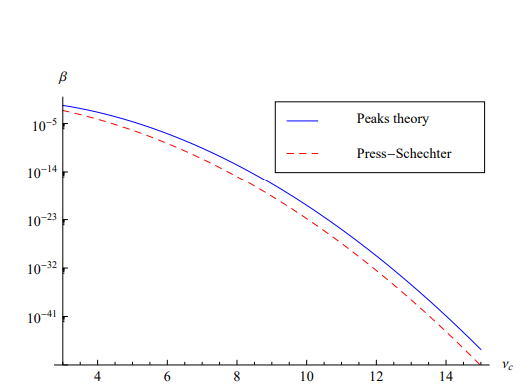
\includegraphics[width=0.7\textwidth]{Peaksvspress.png}
    \caption{The  Value of $\beta$ calculated using Press-Schechter or Peaks theory against $\nu_c = \delta_c/\sigma$. Taken from \cite{Young_2014} }
    \label{fig:3.1}
\end{figure}

Figure \ref{fig:3.1} illustrates the difference between the predicted values for each computation. While $\nu$ is not too large, the two are in fairly close agreement (varying by a factor of order 10). The difference between $\beta {peaks}$ and $\beta_{PS}$ is consistently higher for larger values of $\nu_c$. The error caused by the uncertainty in the threshold value $\delta_c$, however, overpowers the difference between both methods.\\
The mass variance in radiation domination(w = 1/3) is given by
\begin{align}
    \sigma^{2}(R) = \frac{16}{81} \int_{0}^{\infty} \,\frac{dk}{k}  \Tilde{W}^{2}(R,k) (kR)^4\mathcal{P}_{\mathcal{R}_{c}}(k).  \label{3.34}
\end{align}
where $ \Tilde{W}^{2}(R,k)$ is the Fourier transform of the window function used to smooth the density contrast on a comoving scale R($\approx 1/(a_{form} H_{form}) = 2GM/a_{form} \gamma^{_1}$),$\mathcal{P}_{\mathcal{R}_{c}}(k)$ is the power spectrum of the primordial comoving curvature perturbation. We saw before that the power spectrum explains the amplitude of the density perturbations on different scales at some initial time. We define a "Transfer function"\footnote{Appendix \ref{Transfer function}} that modifies this primordial power spectrum and describes the evolution of the density perturbations on subhorizon scales.  So we can re-write Eq.\ref{3.34} as
\begin{align}
    \sigma^{2}(R) = \frac{16}{81} \int_{0}^{\infty} \,\frac{dk}{k}  \Tilde{W}^{2}(R,k) (kR)^4\mathcal{P}_{\mathcal{R}_{c}}(k) T^{2}(kR/\sqrt{3}).  \label{3.35}
\end{align}
We assume $\sigma(R) \ll 1$ which enables us to translate the constraint on $\beta$ into the constraint on $\nu_{c}$ which corresponds to the amplitude of the density fluctuation from the above equation. It would also provide directions for creating successful inflationary models with PBH formation. For example, if the constraint on $f$ for $30 M_\odot$ would be obtained as $f_{pbh} < 10^{-3}$, which is equivalent to $\beta < 3 \times 10^{-11}$ it could be interpreted as $\nu_{th} \gtrsim 6.46$, that is , that is, $\sigma \lesssim 0.08$ with $\delta_{c} = 0.5 $.
% \section{Monochromatic vs Extended}
% In the previous discussion to find the abundance of PBH, we considered a monochromatic mass function which serves as a good starting point for considering models which have a narrow spread of mass like the axion-curvaton model \cite{Kasuya_2009}. However, in a more realistic situation, the analysis can be extended to the case in which the PBH has an extended mass spectrum. An approach to represent it as shown in Ref. \cite{Carr:2016drx} is to integrate the differential mass function $\dv{n}{M}$ over a mass window of width $M$ at each $M$, which gives us the continuous function
% \begin{align}
%     n(M) =  M \dv{n}{M} = \dv{n}{ln M} \label{3.36}
% \end{align}
% $n(M)$ is interpreted as the number density of the PBHs in the mass range$(M,2M)$. We can define the quantities corresponding to the mass density and dark-matter fraction, respectively, in the same mass range as
% \begin{align}
%     \rho(M) = M^{2} \dv{n}{M} , f(M) = \frac{\rho(M)}{\rho_{CDM}} \label{3.37}
% \end{align}
% This has the advantage of allowing one to see where the majority of the mass is right away and is analogous to splitting the mass up into bins. If the width of the mass function is less than M, the aforementioned representations are problematic. We have seen that one can always specify an effective value $f(M)$ at each mass scale if one considers an extended mass function to be one with a width greater than $M$. Although it is simple if the mass function is a delta function (ie. exactly monochromatic), the issue for monochromatic mass functions is typically more challenging. If it is almost monochromatic, or if its width is $(\Delta (M) \ll M)$, then there is an issue.\\
% The mass function should only be very extended if the PBHs are formed from precisely scale-invariant density fluctuations, even if a perfectly monochromatic mass spectrum is obviously not physically feasible. This has the critical implication that a constraint on one mass scale may also imply a constraint on nearby scales. We noted that the monochromatic assumption fails miserably if PBHs develop through critical collapse, and Ref \cite{Yokoyama:1998xd} has discussed how this modifies the shape of $\beta(M)$.
%%%%%%%%%%%%%%%%%%%%%%%%%%%%%%%%%%%%%%%%%%%%%%%%%%%%%%%%%%%%%%%%%%%%%%%%%%%%%%%%%%%%%%%%%%%%%%%%%%%%%%%%%%%%%%%%%%%
\section{Models of Inflation for PBH generation}
In the previous chapter, we discussed how inflation provides a mechanism for generating primordial perturbations via quantum fluctuations of a scalar field and the aspects which are relevant to the formation of PBH. In the standard single slow-roll inflation, the slow-roll parameter is anticipated to suppress the higher-order cumulants. However, non-standard inflationary models that violate the slow-roll condition must be taken into consideration for effective PBH formation which will be discussed in this section.\\
We have observed that PBH arises when an overdense region enters the Hubble horizon. If these regions are sourced by the primordial curvature perturbations, then the size of the overdense region should be determined by the comoving wavenumber, $k$ of the primordial perturbations. So, we can obtain a relation between the Hubble Scale at the PBH formation and the comoving wavenumber of the sourced primordial curvature perturbation as $k =aH_{|formation}$.
During radiation era $aH \propto a^{-1}$, hence we can write the relation between comoving wave number and the Hubble parameter at the formation as $H_{form} \propto k^2$, which we can substitute in the Eq. \ref{3.12} for $M$. So, we get a relation between the mass of PBHs and the comoving wavenumber as \cite{Sasaki_2018}


\begin{align}
    M(k) & =\left.\gamma \frac{4 \pi}{3} \rho H^{-3}\right|_{k=a H} =\gamma M_{eq}\left(\frac{g_{* eq}}{g_*}\right)^{1 / 6}\left(\frac{k_{eq}}{k}\right)^2 \label{3.36}
\end{align}

where $M_{eq}$ denotes the horizon mass at the matter radiation equality calculated as,
\begin{align}
    M_{eq}=\frac{4 \pi}{3} \rho_{eq} H_{eq}^{-3}=\frac{8 \pi}{3} \frac{\rho_r^0}{a_{eq} k_{eq}^3} \label{3.37}
\end{align}

We have used an approximation that the effective d.o.f. for energy density $g_*$ is almost equal to that for entropy density $g_{*s}$. Using $\rho_r^0=7.84 \times 10^{-34}g cm^{-3}$, $k_{eq}=0.07 \Omega_k h^2 Mpc^{-1}, a_{eq}^{-1}=24000 \Omega_k h^2$, and $g_{eq}=$ 3.36, we can finally obtain 
\begin{equation}
    M(k)=30 M_{\odot}\left(\frac{\gamma} {0.2}\right)\left(\frac{\left.g_*\right|_{k=a H}}{106.75}\right)^{-1 / 6}\left(\frac{k}{2.9 * 10^{5} Mpc^{-1}}\right)^{-2} \label{3.38}
\end{equation}
Inferring precedence between the observable scales via CMB measurements and $30 M_{\odot}$ PBHs from the above equation using the pivot scale as mentioned in Planck 2015\cite{Planck:2015fie} as a typical observable scale by CMB observations, $k_{CMB}$ we see that
\begin{align}
    \mathcal{N}_{CMB -30M{\odot} PBHs} = \ln\qty(\frac{k_{30M_{\odot} PBHs}}{k _{CMB}}) = \ln \qty(\frac{2.9 \times 10^{5} \text{Mpc}^{-1}}{0.002 \text{Mpc}^{-1}}) \sim 20, \label{3.39}
\end{align}

On the other hand, it is necessary for there to be a minimum of 50-60 e-folds between the time the existing horizon scale leaves the Hubble horizon and the end of inflation.
As a result of the preceding discussion, we infer that if we wish to create $30M_{\odot}$ PBHs from the perturbations of the primordial density, we need to take into account any mechanism that can amplify the perturbations during the inflationary phase.


%%%%%%%%%%%%%%%%%%%%%%%%%%%%%%%%%%%%%%%%%%%%%%%%%%%%%%%%%%%%%%%%%%%%%%%%%%%%%%

\subsection{Single Field Inflation}
In the standard slow roll inflation scenario the power spectrum form is written as \ref{2.148} (with the parameters $\alpha_s$ and $\beta_s$ suppressed) as:
\begin{align}
    \mathcal{P}_{\mathcal{R}_c}(k) = A_{\mathcal{R}_c}\qty(\frac{k}{k_{*}})^{n_s - 1}, \ \label{3.40}
\end{align}
where $n_s -1 $ can be written in terms of the slow-roll parameters( $\eta$ (Eq.\ref{2.36}) and $\epsilon$ (Eq.\ref{2.41})) as shown in Eq. \ref{2.149}.
For successful inflation, the condition to be satisfied is $\eta,\epsilon \ll 1$. Let us see if the spectral index satisfies the condition. \\
From the latest CMB observation, it is indicated that $P_{R_c} \approx 10^{-9}$(COBE normalization) over the CMB observable scales and the effects of PBH formation is quite effective to have a point of interest for  $\mathcal{P}_{\mathcal{R}_c}  = \mathcal{O}(10^{-2} - 10^{-1})$. So, for realizing such a large amplitude at $k = k_{30M_{\odot} PBHs} = 2.9 \times 10^5 \mathrm{MPc^{-1}}$ with a blue tilted power spectrum (large amplitude for small scale i.e large comoving number) consistent with the COBE normalization, we need \cite{Sasaki_2018}

\begin{align}
    n_s - 1 = \ln \qty(\frac{\mathcal{P}_{\mathcal{R}_c}(k_{30M{\odot} PBHs})}{\mathcal{P}_{\mathcal{R}_c}(k_{CMB})})/ \ln\qty(\frac{k_{30M_{\odot} PBHs}}{k_{CMB}}) \simeq 0.85 \label{3.41}
\end{align}
From the obtained value we observe that the spectral index value obtained from CMB observations like the Planck observation, we have 
\begin{align}
    n_s = 0.968 \pm 0.006 \text{at} k_{*} = 0.05 \mathrm{Mpc^{-1}}\label{3.42}
\end{align}
Hence, for PBH the standard inflationary model conflicts with the CMB observations even if we implement the blue-tilted power spectrum.

%%%%%%%%%%%%%%%%%%%%%%%%%%%%%%%%%%%%%%%%%%%%%%%%%%%%%%%%%%%%%%%%%


\subsection{Running  Mass Inflation}
 The formation of PBH in the running mass inflation model is one of the possibilities to realize a relatively large blue-tilted inflationary model consistent with the Planck results. the inflationary potential is defined in this case as 
 \begin{align}
     V(\varphi) = V_{0} + \frac{1}{2}m_{\varphi}^{2}(\varphi)\varphi^{2} \label{3.43}.
 \end{align}
The significant dependency of the $\eta$ on time during inflation in this model suggests that the scale dependence of the $n_s$ may also become large. Thus, when $\eta$ remains to be small to be consistent with the Planck result on CMB scales, but $\eta$ takes a positive larger value on smaller scales, we can realize the large
 amplitude of primordial curvature perturbations on an appropriately small scale which could be seeds of PBHs. The primordial power spectrum for these types of models incorporates the scale-dependence of the spectral index perturbatively rather than being a simple power law as mentioned in Eq. \ref{2.148}. Let us rewrite it below
 \begin{align}
    \mathcal{P}_{\mathcal{R}_c}  = A_s (\frac{k}{k_0})^{n_s -1 + \frac{1}{2}\alpha_{s} ln(k/k_0)+ \frac{1}{3!}\beta_{s}ln^2(k/k_0) + ....}, \label{3.44} 
 \end{align}
Where $\alpha_{s}$ and $\beta_{s}$ are the "running spectral index" and "running of running" parameters, which are greatly suppressed during slow-roll inflation but are very significant in this model. Ref. \cite{Sasaki_2018} discussed that for the above parameterization to produce $30M_{\odot} \mathrm{PBHs}$\footnote{Focusing on inflation models producing PBHs of $\mathcal{O}(1-10)M_{\odot}$} with $n_s = 0.968$ on CMB scales, $\alpha_{s}$ needs to be taken to be about 0.1.
 It was further addressed that for such a large $\alpha_{s}$ and assuming negligibly small $\beta_s$, PBH with smaller masses would be overproduced. To avoid this overproduction a cutoff in the primordial power spectrum at an appropriate scale is needed, which is realized by taking into account the non-negligible "running of running" parameters $\beta_s$. 
%%%%%%%%%%%%%%%%%%%%%%%%%%%%%%%%%%%%%%%%%%%%%%%%%%%%%%%%%%%%%%%%%%%%%%%%%%%%%%%%%%%%%%%%%%%%%


\subsection{Multifield}
In this section, we will briefly discuss some multi-field scenarios that can generate large primordial curvature perturbations with large amplitudes.
\subsubsection{Double Inflation}
A peak in the primordial power spectrum can be realized at an appropriate scale if the inflaton experiences a period during inflation where it temporarily slows down. This corresponds to a very flat region in the inflationary potential, as we have mentioned in the single-field inflation scenario. The temporal violation of the conventional slow-roll conditions is crucial in the aforementioned models for realizing the enhancement of primordial curvature perturbations to form PBHs during the inflationary era. This case of features can be readily achieved in the Multi-Scalar models. In double inflation, there are two separate periods of inflation, with
perturbations on cosmological scales being generated during the first period and those on small scales during the second. Hybrid inflation models with a mild waterfall transition, which will be discussed next, fall into this class. 
\subsubsection{Hybrid Inflation}
A detailed description of Hybrid inflation can be found in reference \cite{PhysRevD.54.6040} \cite{PhysRevD.92.023524}. Hybrid inflation is the most commonly studied two-field model in the context of PBH production. $\varphi$ is one of the fields that slow-rolls whereas the other field $\psi$'s false vacuum energy  drives the accelerated expansion. There is a phase transition that takes place at a critical value of $\varphi$ with $\psi$ undergoing a waterfall transition to a global minimum and the inflation stops. There are large quantum fluctuations around the phase transition which generates spikes in the power spectrum on small scales, which leads to a large abundance of light PBH. There can be some parameter values for which the waterfall transition is 'mild' so that there is a 2nd phase of inflation as the field $\psi$ evolves to the minimum of its potential. In this instance, isocurvature perturbations are produced at the first stage of the waterfall transition, when both fields are significant, and this causes a large peak in the curvature perturbation power spectrum. At the first stage of inflation, perturbations on cosmological scales are produced and may be consistent with CMB observations.\\


\subsubsection{Curvaton Model}
For producing primordial curvature disturbances that can result in the production of primordial black holes, the curvaton scenario offers an alternative to the single field inflationary model (PBHs). The inflaton, which causes inflation, and the curvaton, which causes the perturbations in primordial curvature, are the two scalar fields involved in the curvaton scenario. As the curvaton field begins to oscillate and behave as non-relativistic matter during the radiation-dominated epoch, the curvaton field initially causes isocurvature perturbations, which eventually turn into adiabatic curvature perturbations. The adiabatic curvature perturbations become constant in time when the curvaton eventually decays into radiation\cite{Lyth_2005}. In order to produce the huge amplitude fluctuations required for PBH creation on small scales while maintaining consistency with the CMB measurements on larger scales, the curvaton fluctuations exhibit a scale-invariant feature on smaller scales and a cutoff on a larger scale. On super-Hubble scales, multiple curvaton fields can intensify the curvature perturbations, producing a large number of PBHs up until the enhancement stops. For example "axion-like curvaton\cite{PhysRevD.87.063519}".











%%%%%%%%%%%%%%%%%%%%%%%%%%%%%%%%%%%%%%%%%%%%%%%%%%%%%%%%%%%%%%%%
%%%%%%%%%%%%%%%%%%%%%%%%%%%%%%%%%%%%%%%%%%%%%%%%%%%%%%%%%%%%%%%%
%%%%%%%%%%%%%%%%%%%%%%%%%%%%%%%%%%%%%%%%%%%%%%%%%%%%%%%%%%%%%%%%




\section{Exploring Limitations in Simplified Models of Primordial Black Hole Formation} \label{limtiation}
In our previous discussion to find the abundance of PBH, we considered a monochromatic mass function with a mass similar to the horizon mass at the creation and that the PBHs arise from the collapse of overdensities that are spherical and have a Gaussian distribution which serves as a good starting point. However, this oversimplified model can result in misinterpretation of observational constraints. As a result,  a more realistic portrayal of the formation process is required, especially as the constraints on the allowed PBH density at each epoch have become more precise. Additionally, The potential existence of intermediate-mass PBHs has also been suggested by recent observations \cite{2016PhRvL.116t1301B}, which emphasizes the need for a more exact description of PBH production.
\subsection{Precise Threshold Value}
The estimated threshold density perturbation for PBH formation is approximately 1/3 according to Eq. \ref{3.8}, but more precise values have been obtained through extensive research involving numerical simulations and analytical calculations. A formula in Ref. \cite{Harada_2013} gives a close estimate of the threshold as
\begin{align}
    \Tilde{\delta}_c =[3(1+w)/(5+3w)] \sin ^2[\pi \sqrt{w} /(1+3 w)], \label{3.45}
\end{align}
where $\Tilde{\delta}_c$ is the amplitude measure used in
numerical simulations and
\begin{align}
    \delta_{H c}^{UH}=\sin ^2[\pi \sqrt{w} /(1+3 w)] ,\label{3.46}
 \end{align}
 where $\delta_{H c}^{UH}$ is the amplitude of the density perturbation at horizon crossing in the uniform Hubble slice and $w$ is the equation of state of the dominant component in the Universe at the formation. However, it has been found that the threshold is not fixed as different density or curvature perturbation profiles can collapse to form PBHs above different thresholds, which makes physical sense. The range of the threshold's spread, measured in terms of the comoving density perturbation, is from 0.3 to 0.66. It's interesting to note that the rough estimate of 1/3 is included in this range.
 %%%%%%%%%%%%%%%%%%%%%%%%%%%%%%%%%%%%%%%%%%%%%%%%%%%%%%%%%%%%%%%%%%%%%%%%%%%%%%%%%%
 \subsection{Critical Collapse}

\hspace{0.5cm}Previously, it was assumed that an overdensity that enters the horizon and collapses to a black hole with a mass of the order of the horizon mass $M_{H}$ would do so immediately. However, it has since been shown that when considering spherical symmetry, the relationship between the black hole mass $M_{BH}$ and the overdensity $\delta$ at horizon crossing and the horizon mass $M_{H}$ follows a critical scaling relation described by equation 
 \begin{align}
     M_{BH} = \kappa M_{H}(\delta -\delta_{c})^\gamma \label{3.47},
 \end{align} 
 This scaling relation includes a constant $\kappa$, a threshold overdensity $\delta_{c}$, and a critical exponent $\gamma$ that depends on the fluid containing the overdensity at horizon crossing \cite{Musco_2013}. The scaling relation in Eq. \ref{3.47} was confirmed  through numerical work in Ref. \cite{Musco_2013}. They also showed that the critical exponent $\gamma$ is independent of the perturbation profile, however, $\delta_{c}$ and $\kappa$ may depend on the perturbation profile.\\

When applying this critical collapse model to primordial black hole formation, it was found that the horizon-mass approximation was still valid at the time of formation. However, this conclusion was based on the assumption that the primordial black hole mass function was monochromatic. Further study has revealed that the inclusion of critical collapse can cause a significant shift, lowering, and broadening of the primordial black hole mass spectra by several orders of magnitude when a realistic model of the power spectrum underlying their production is taken into account. These small effects should be taken into account to obtain precise constraints on inflationary models. This has been demonstrated for a variety of inflationary models in Ref. \cite{K_hnel_2016}.
%%%%%%%%%%%%%%%%%%%%%%%%%%%%%%%%%%%%%%%%%%%%%%%%%%%%%%%%%%%%%%%%%%%%%%%%%%%%%%%%%%%%%%%
\subsection{Non-sphericity of the Overdense Region}
In our previous discussion, we considered an isolated spherically symmetric perturbation as a criterion for PBH formation, which is a reasonable first approximation and makes our calculation easier. In reality, this is not the case and the effects of non-sphericity might be consequential even if in most cases the initial non-sphericity is either small or eventually leads to spherical objects. One of the most simple and spherically deviated overdense regions is approximated as an ellipsoid. The approximate threshold value for ellipsoid collapse is 
\begin{align}
    \frac{\delta_{ec}}{d_c} = 1 + \kappa \qty(\tall \frac{\sigma^2}{\delta_{c}^2})^{\gamma} \label{3.48}
\end{align}
where $d_c$ is the threshold for the spherical collapse,$\sigma^2$ is the amplitude of the density power spectrum at a given scale, and $\kappa$ and $\gamma$ are constants to be found numerically.
\cite{Kuhnel:2016exn}, it was stated that to estimate the modification of the threshold in the case of the non-spherical overdense region that was approximated as an ellipsoid, it was demanded that a spherical region enclosed by the shortest axis of the ellipsoid satisfies the collapse criterion for the spherical overdensity. The collapse along the longer axes follows, moving faster than linearly, as the collapse condition. They considered a Gaussian-distributed overdensity and showed that the expectation value for the shape of densities as
\begin{align}
    \langle e \rangle = \frac{3\sigma}{\sqrt{10\pi} \delta}\label{3.49}
\end{align}
Furthermore, they assumed that the ellipsoid is of uniform density and that the density profile in the central region is higher. Thus, given this simplistic analysis, they discover that$\gamma = 1/2 $ and $\kappa = (9\pi \sqrt{10})$.
They discovered that the non-sphericity effects would raise the formation threshold, which would suppress the mass spectrum generally. Although the exact amount of non-sphericity-related suppression is unsure, the mass spectrum's functional shape remains unaltered. However, it should be noted that  Eq. \ref{3.49}, does not provide the ellipticity for non-Gaussian overdensities, therefore it is important to consider how these two effects interact.

%%%%%%%%%%%%%%%%%%%%%%%%%%%%%%%%%%%%%%%%%%%%%%%%%%%%%%%%%%%%%%%%%%%%%%%
\subsection{Non-Linear effects}

The energy density profile in Eq. \ref{3.4} for radiation dominated universe($w = 1/3$) can be (re)written as
\begin{align}
    \delta(\vec{x}, t)=-\frac{4}{9} (\frac{1}{aH})^{2} e^{-2 \zeta(\vec{x})}\left[\nabla^2 \zeta(\vec{x})+\frac{1}{2} \partial_i \zeta(\vec{x}) \partial^i \zeta(\vec{x})\right] \label{3.50}
\end{align}
We can notice from the above equation that the relation between the overdensity and the curvature perturbation is intrinsically non-linear and we obtain a linear relation only under the condition that both the $\zeta$-curvature and curvature gradients are small $\left(\left|\zeta\right|,\left|\nabla \zeta\right| \ll 1\right)$. In particular, in Eq  \ref{3.50} it is often assumed that the exponential damping $e^{2 \zeta}$ (effects the peak of the profile) and the quadratic gradient correction $\left(\nabla \zeta \cdot \nabla \zeta\right)$ (effects the tail of the profile) can be neglected, effectively linearising the relation between $\zeta$-curvature perturbation and the overdensity perturbation $\delta^{\text {LIN }} \propto \nabla^2 \zeta$


Even if the linear approximation is accurate at the beginning, non-linearities have already had a big impact by the time the horizon is crossed since both curvature and overdensity perturbations are of order unity. When assessing PBH abundance, numerical simulations of PBH formation and  cosmological connections, neglecting the non-linearities have a substantial impact. This topic has been extensively covered by Kalaja \emph{et al}\cite{Kalaja:2019uju}. \\
They demonstrate that, depending on the shape of the perturbation, applying a linear approximation significantly underestimates the real size of the perturbation (and hence the mass contained in the horizon) by a factor of up to $\sim$ 6: Most noticeably impacted are perturbation profiles that are steeper. \\
They also compare some key quantities with the full non-linear equation(NL)  with their corresponding linear approximation(LIN). For example, they showed that  linearisation underestimates the typical scale of perturbation. Under linear approximation, the typical scale of the perturbation is $r_t^{\mathrm{LIN}}=\hat{r}_k$, which is to be compared against the typical non-linear scale $r_t^{\mathrm{NL}}=\hat{r}_k e^{-\zeta\left(\hat{r}_k\right)}$. Since $\zeta$ is negative, linearisation underestimates the real size of the perturbation, i.e., $r_t^{\mathrm{LIN}} / r_t^{\mathrm{NL}}<1$. \\
Now, since in radiation-domination the comoving horizon scales as $r_{\text {H }} \propto t^{1 / 2}$ and the horizon crossing condition is $a_k H_k r_t=1$, linearisation also underestimates the horizon crossing time $t_k$  and since the inferred mass of the PBH is also affected by linearisation through a different estimate of the horizon crossing time as seen in Eq. \ref{3.47} where $M_{H}(t) = (2H)^{-1}$, the main effect is that the linear approximation underestimates the mass inside the horizon:
\begin{align}
    \frac{M_{\text {hor }}^{\mathrm{LIN}}}{M_{\text {hor }}^{\mathrm{NL}}}=\frac{t_k^{\mathrm{LIN}}}{t_k^{\mathrm{NL}}}=\left(\frac{r_t^{\mathrm{LIN}}}{r_t^{\mathrm{NL}}}\right)^2<1 .\label{3.51}
\end{align}
Another significant aspect that was highlighted was the importance of nonlinearity in the smoothing process.
To account for spatial curvature, which introduces certain nuances, it is advised that filtering be done in physical coordinates rather than comoving coordinates, as in linear theory. However, when the spatial curvature is introduced into the filtering procedure, and the full non-linear relation between the non-linear overdensity and curvature is used, filtering the overdensity fields or curvature is no longer equivalent, implying that filtering $\zeta$ is not equivalent to filtering $\delta$ in the non-linear case. Furthermore, it was discussed that because of the non-linearity between overdensity and curvature, the two-point functions of the overdensity field receive contributions from all of the n-point functions of the $\zeta$ -curvature field, implying the importance of non-Gaussianity when going beyond the linear approximation. (For more details refer to Ref. \cite{Kalaja:2019uju}). 
%%%%%%%%%%%%%%%%%%%%%%%%%%%%%%%%%%%%%%%%%%%%%%%%%%%%%%%%%%%%%%%%%%%%%%%%%%%%%%%%%%%%%%%%%
\subsection{Non-Gaussianity}
PBHs are formed from the extremely high-density tail of the spectrum of fluctuation, and their abundance is significantly affected by any  non-gaussianity in the density perturbation profile.
The way the perturbations are created, which is determined by the inflationary models, determines the impact of non-Gaussianity on the calculation of the perturbations to the primordial curvature and can alter the initial mass fraction PBHs in a major way.\\
 
In this section, we will follow Ref. \cite{Franciolini:2018vbk}  where they discuss the role of non-gaussianity in determining the PBH mass-fraction at formation time by using a path integral formulation \cite{Matarrese:1986et}. However, instead of going into too much detail, we will focus on discussing the main findings and results of the study(for detailed calculation refer to \cite{Franciolini:2018vbk}).

The probability for a single-density contrast  $\zeta_{R}$ to be above the threshold $\zeta_{c}$ for it to collapse and form a black hole can be directly calculated by evaluating the one-point threshold statistics and it is given by
\begin{align}
    P\left(\zeta_{R}>\zeta_{c}\right)=\left\langle\rho_{\nu, R}(\vec{x})\right\rangle & =\left\langle\Theta\left(\zeta_{R}(\vec{x})-\nu \sigma_{R}\right)\right\rangle = h_{0}(\nu)+\frac{e^{-\nu^{2} / 2}}{\sqrt{2 \pi}} \sum_{n=3}^{\infty} \frac{1}{2^{\frac{n}{2}} n !} \Xi_{n}(0) H_{n-1}\left(\frac{\nu}{\sqrt{2}}\right), \label{3.52}
\end{align}
for a more detailed description refer to Ref. \cite{Franciolini:2018vbk, Matarrese:1986et}.
Eq. \ref{3.52} is the exact solution without any approximations. For large threshold, i.e $\nu \gg 1$ using the asymptotic behaviour of Hermite polynomials and the complementary error function 
\begin{align}
    \begin{aligned}
        & H_{n}\left(\frac{\nu}{\sqrt{2}}\right)=2^{\frac{n}{2}}                \nu^{n}\left(1+\mathcal{O}\left(\nu^{-2}\right)\right) \\
        & h_{0}(\nu)=\frac{1}{2} \operatorname{Erfc}\left(\frac{\nu}{\sqrt{2}}\right)=\frac{e^{-\nu^{2} / 2}}{\sqrt{2 \pi \nu^{2}}}\left(1+\mathcal{O}\left(\nu^{-2}\right)\right),\label{3.53}
    \end{aligned}
\end{align}
Eq. \ref{3.52} reduces to
\begin{align}
    P\left(\zeta_{R}>\zeta_{c}\right)=\frac{e^{-\nu^{2} / 2}}{\sqrt{2 \pi \nu^{2}}} \exp \left\{\sum_{n=3}^{\infty} \frac{(-1)^{n}}{n !} w_{R}^{(n)}(0) \nu^{n}\right\}=\frac{1}{\sqrt{2 \pi \nu^{2}}} \exp \left\{-\nu^{2} / 2+\sum_{n=3}^{\infty} \frac{(-1)^{n}}{n !} \xi_{R}^{(n)}(0)\left(\zeta_{c} / \sigma_{R}^{2}\right)^{n}\right\}, \label{3.54}
\end{align}

The argument (0) signifies that all the points have to be taken coinciding with each other. On taking the smoothing radius to be $R_{H}$ we can see that the expression gives the primordial mass fraction $\beta$ with the approximation of $\nu \gg 1$. Another interesting thing to notice is that, when the higher order $(n > 2)$ linked correlators vanish, it is possible to identify the leading order term that produces the Gaussian outcome.
Let's now look at how Eq. \ref{3.54} is used to analyze the effects of non-Gaussianity and how important it is to evaluate whether higher-order correlators that incorporate the non-Gaussian corrections are significantly impacting the computation of abundance in a given model.\\
Taking inspiration from the notion of fine-tuning we see how sensitive $\beta(M)$ is to the various dimensionless quantities, the cumulants, which are defined by the relation
\begin{align}
    S_n=\frac{\xi_{\nu, R_H}^{(n)}(0)}{\left(\xi_{\nu, R_H}^{(2)}(0)\right)^{n-1}}=\frac{\langle\overbracket{\zeta_{R_H}(\vec{x}) \cdots \zeta_{R_H}(\vec{x})}^{n \text {-times }}\rangle}{\sigma_{R_H}^{2(n-1)}}, \label{3.55}
\end{align}
Now, the fine-tuning parameter $\Delta_{n}$ which is the logarithmic variation of the PBH abundance after introducing the n-th cumulant is defined as
\begin{align}
    \Delta_{n}=\frac{\mathrm{d} \ln \beta_{\operatorname{prim}}(M)}{\mathrm{d} \ln S_{n}} \label{3.56}
\end{align}
In the presence of the $n^{th}$ cumulant, the non-Gaussian PBH abundance Eq. \ref{3.52} is related to the Gaussian abundance in terms of the correction parameter as
\begin{align}
    \frac{\beta_{\text {prim }}^{\mathrm{NG}}(M)}{\beta_{\text {prim }}^{\mathrm{G}}(M)}=e^{\Delta_{n}} ,\label{3.57}
\end{align}
From the above Eq. \ref{3.57} we can tell that the resulting PBH abundance is exponentially sensitive to deviation from Gaussianity unless 
$
\left|\Delta_{n}\right| \lesssim 1
$
\\

Using, the Gaussian mass fraction $\beta_{G} \simeq \sqrt{\frac{1}{2\pi\nu^{2}}}e^{-\nu^{2}/2}$ and Eq. \ref{3.54} we find that
\begin{align}
    \left|\Delta_{n}\right|=\frac{1}{n !}\left(\frac{\zeta_{c}}{\sigma_{R_{H}}}\right)^{2}\left|S_{n}\right| \zeta_{c}^{n-2} \label{3.58}
\end{align}
The above equation demonstrates that non-Gaussianity modifies the Gaussian prediction for the PBH abundance exponentially unless
\begin{align}
    \left|S_{n}\right| \lesssim\left(\frac{\sigma_{R_{H}}}{\zeta_{c}}\right)^{2} \frac{n !}{\zeta_{c}^{n-2}} \label{3.59}
\end{align}
Franciolini \emph{et al}\cite{Franciolini:2018vbk} analysed the restrictiveness of the above condition Eq. \ref{3.59} in the case of PBH from the single field inflation model and the axion-curvaton model(presence of a spectator field). Following Ref. \cite{Motohashi:2017kbs}, they set $\beta(M)$ to correspond to the total amount of dark matter that exists today in the form of PBHs and look for the effects of non-Gaussianity. They find the non-Gaussian results in the cases of the single-field model and the axion-curvaton model are smaller by about ten and twenty orders of magnitude respectively than the Gaussian results, indicating the sensitivity of the cosmological predictions to the non-Gaussianity. Their findings further demonstrate how non-Gaussian corrections affect the PBH's clustering features, which in turn influences PBH merger and may have an impact on PBH cosmic evolution.




    



,